% !TEX root = ../spec_kernel_agent_main.tex

\begin{figure}[t]
    \centering
    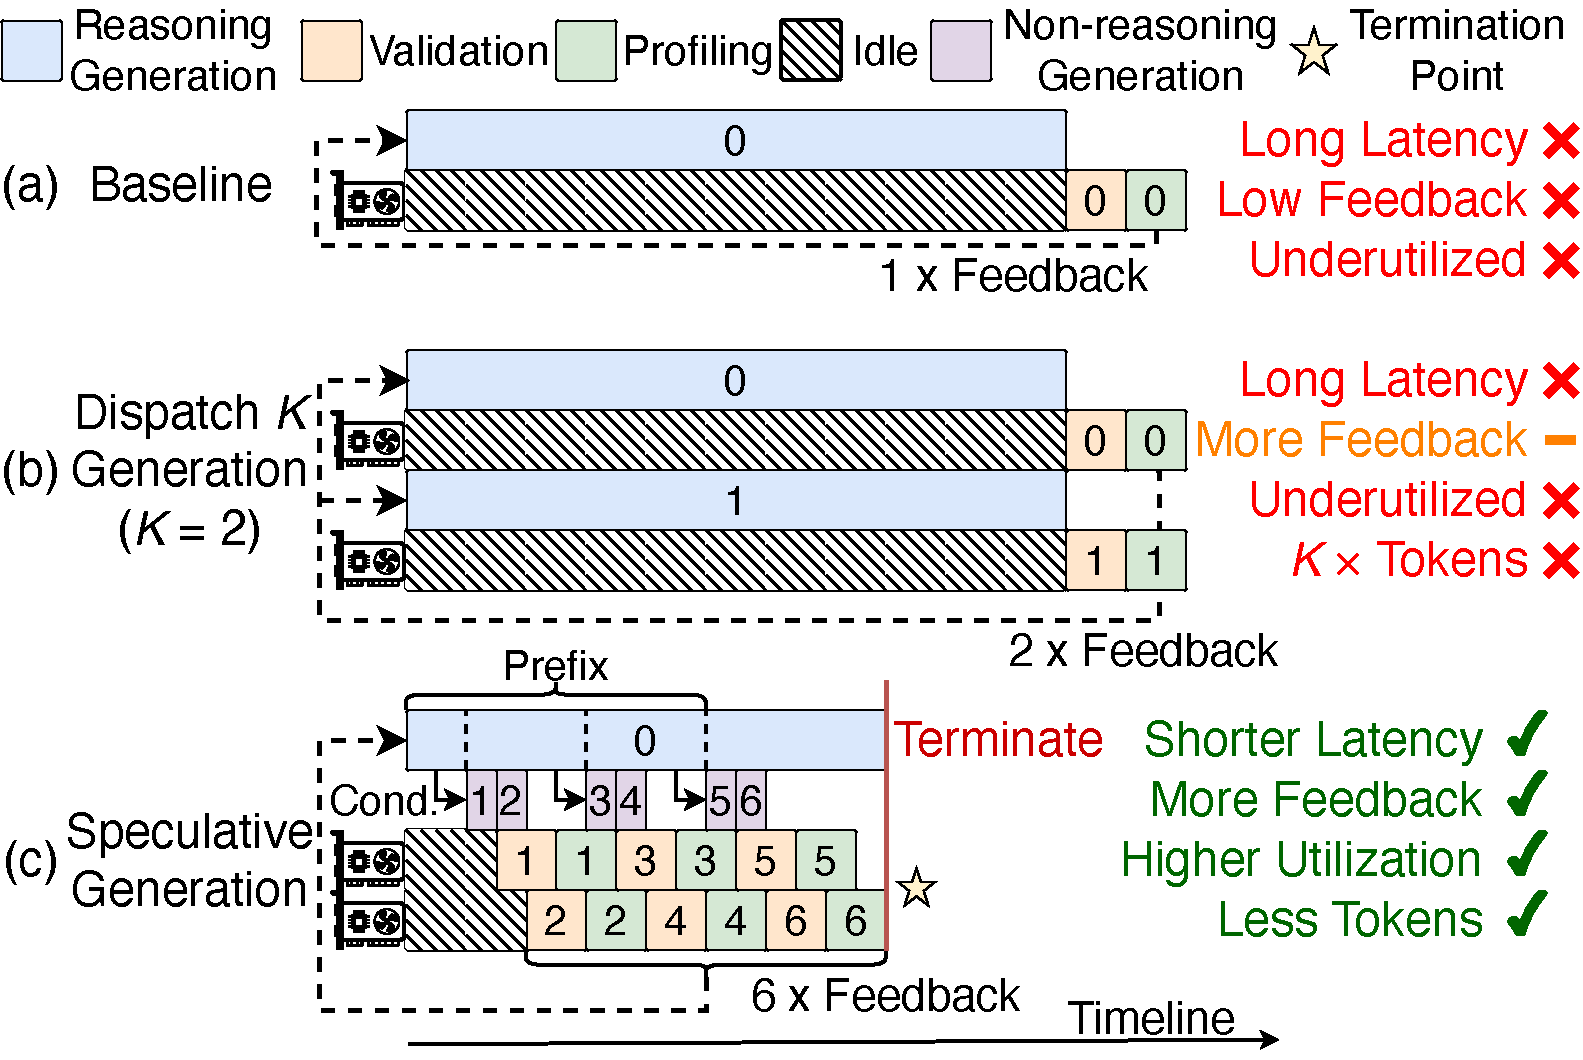
\includegraphics[width=\linewidth]{figs/long_abstract.pdf}
    \vspace{-20pt}
    \caption{Comparison of existing techniques in agentic kernel optimization and speculative generation.}
    \vspace{-15pt}
    \label{fig:timeline_workflow}
\end{figure}


\section{Design Insight and Challenges}\label{sec:challenges}

\subsection{Limitations of Prior Systems}\label{subsec:limitations_of_prior_systems}

As illustrated in \S\ref{sec:mot}, the baseline iterative refinement framework~\cite{kernelbench}, which performs one generation per iteration (see Figure~\ref{fig:timeline_workflow}(a)),
suffers from three system-level inefficiencies.
An intuitive approach is to dispatch multiple generations per iteration to improve search efficiency.
However, (1) dispatching multiple \emph{reasoning generations}~\cite{cudaforge,K-Search,kernelagent2025,AlphaEvolve,Kernel-Smith} 
roughly multiplies the token cost by $K$ (see Figure~\ref{fig:timeline_workflow}(b)).
The candidate kernels become actionable only after the reasoning process finishes, 
resulting in significant idle time for validation/profiling resources.
(2) Dispatching multiple \emph{non-reasoning generations} reduces both generation latency and token cost but rarely produces valid or performant kernels.
Table~\ref{tab:nonreasoning_speedups_w_wo_shared_prefix_cache} shows that 8/10 tasks on GLM 
and 4/10 tasks on DeepSeek fail to produce any valid kernels after 100 iterations of non-reasoning generations.

% Compared with the baseline \texttt{KernelBench}~\cite{kernelbench} iterative refinement framework, which performs one generation per iteration (see Figure~\ref{fig:timeline_workflow}(a)),
% prior systems share a common approach of dispatching $K$ reasoning generations per iteration to produce more profiling feedback (Figure~\ref{fig:timeline_workflow}(b)).
% This approach roughly multiplies the token cost by $K$.
% A strawman alternative is to dispatch non-reasoning generations
% to save token cost. However, non-reasoning generations rarely produce valid or performant kernels. 
% Table~\ref{tab:nonreasoning_speedups_w_wo_shared_prefix_cache} shows that 8/10 tasks on GLM 
% and 4/10 tasks on DeepSeek fail to produce any valid kernels after 100 non-reasoning generations.
% Moreover, these systems do not reduce generation latency since candidate kernels become 
% actionable only after the generation phase finishes, and validation/profiling resources
% remain idle during the reasoning process of the generation phase.

% Prior systems primarily focus on improving the kernel performance by adopting different
% harness engineering strategies~\cite{cudaforge,K-Search,kernelagent2025,AlphaEvolve,Kernel-Smith}.
% However, these systems do not address the three inefficiencies of \S\ref{sec:mot} effectively:
% they dispatch $K$ reasoning generations per iteration to produce more profiling feedback at the cost of 
% roughly $K\times$ token consumption (Figure~\ref{fig:timeline_workflow}(b)). A strawman approach is dispatching non-reasoning generations
% to save token cost. However, non-reasoning generations rarely produce valid or performant kernels. 
% As shown in Table~\ref{tab:nonreasoning_speedups_w_wo_shared_prefix_cache}, 8/10 tasks on GLM 
% and 4/10 tasks on DeepSeek fail to produce any valid kernels with 100 non-reasoning generations.
% Moreover, these systems do not reduce generation latency since candidate kernels become 
% actionable only after the generation phase finishes, and validation/profiling resources still
% remain idle during the reasoning process of the generation phase.

\subsection{Insight: Speculative Generation}\label{subsec:design_insight}
Our key insight is that the reasoning process exposes a window for producing
additional candidate kernels with \emph{reasoning prefix conditioning}.
Since non-reasoning generations are faster than reasoning generations, the system can dispatch
multiple non-reasoning generations in parallel with the ongoing reasoning generation to 
increase the candidate kernel count.
To improve the kernel performance of non-reasoning generations, we condition non-reasoning generations
on the prefix of the reasoning output. Table~\ref{tab:nonreasoning_speedups_w_wo_shared_prefix_cache} shows 
that with this conditioning, non-reasoning generations produce valid kernels on all
tasks and achieve higher speedups. Moreover, because this conditioning shares the reasoning prefix with the reasoning
generation, speculative generations can reuse the prefix cache and reduce token
cost.

\begin{figure}[t]
    \centering
    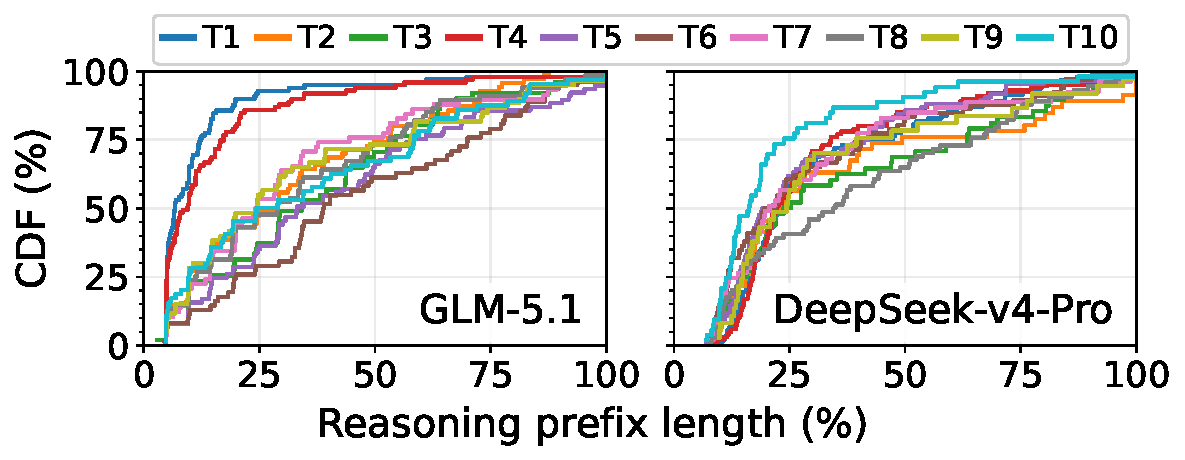
\includegraphics[width=\linewidth]{figs/spec_reach95_token_cdf_dual_GLM_5_1_vs_dsv4_pro.pdf}
    \vspace{-25pt}
    \caption{CDF of the shortest reasoning prefix length for generating a kernel with higher speedups than the average speedup of previously generated kernels across both models.}
    \vspace{-10pt}
    \label{fig:spec_reach95_token_cdf}
\end{figure}
We further explore early termination opportunities with prefix conditioning in Figure~\ref{fig:spec_reach95_token_cdf}.
We record the shortest reasoning prefix that produces a kernel faster than the average of previously generated kernels.
Across GLM-5.1 and DeepSeek-V4-Pro, the prefix length ranges from 14\% to 70\% of the full reasoning trace.
These results show that prefix conditioning can provide useful context for non-reasoning generations 
to produce performant kernels before the full reasoning trace completes.
Once a satisfactory kernel appears,
the system can terminate the reasoning generation early to reduce generation latency. We empirically show that a 
pragmatic termination criterion can reduce generation latency without sacrificing kernel performance 
(see \S\ref{subsec:eval_termination_analysis}).


This insight motivates an iteration-level speculative generation scheme.
Compared with the prior approaches in Figure~\ref{fig:timeline_workflow}(b),
speculative generation in Figure~\ref{fig:timeline_workflow}(c) introduces three benefits:
\textbf{(1)} shorter generation latency by enabling early termination when a
forked kernel meets the termination criterion
\textbf{(C1)};
\textbf{(2)} more profiling feedback via generating more candidate kernels per
iteration
\textbf{(C2)};
\textbf{(3)} higher validation/profiling utilization by keeping
resources busy during the generation phase
\textbf{(C3)}.

\subsection{Challenges of Speculative Generation}\label{subsec:challenges_list}

Realizing speculative generation poses two challenges.

\noindent\textbf{Challenge 1. How to fork and when to terminate.}
Reasoning traces contain noise, such as self-talk and repetition, that disturb
the parsing of useful context for non-reasoning generations.
The system must identify useful conditioning context from a noisy reasoning
trace and decide how many speculative generations to launch.
Too few forks leave validation/profiling resources idle, while too many overload
the queues and delay profiling feedback.
The system should also carefully choose the termination criterion.
Terminating too early sacrifices kernel performance, while
terminating too late saves negligible generation time.

% The system must decide \emph{when} the reasoning prefix provides useful
% conditioning context for non-reasoning generations and \emph{when} to terminate
% the reasoning generation without sacrificing kernel performance.
% The reasoning trace contains kernel-design decisions mixed with noise, such as self-talk and repetition.
% The system should parse the trace to identify when to trigger speculative generations.
% Forking too early wastes speculative tokens on irrelevant context, while forking too late shrinks the number of
% kernels an iteration can produce.
% Terminating too aggressively abandons a still-improving reasoning trace, which must remain a fallback unless a forked
% kernel meets the termination criterion.

\noindent\textbf{Challenge 2. How to manage bursty speculative generation load.}
Speculative generation reshapes the validation and profiling load from sporadic to bursty.
The legacy static ``one GPU per kernel'' partitioning cannot handle this burstiness.
It leaves some GPUs idle while others queue, so resource allocation must adapt as bursts arrive.
% Moreover, the system must also prioritize requests to bound the profiling feedback latency.
Bounding the profiling feedback latency also requires request prioritization.
For local LLM deployments, bursty speculative generations further introduce
additional memory overhead that the system needs to manage.

% The legacy ``one GPU per kernel'' partitioning creates imbalanced utilization.
% For example, one GPU may queue bursty speculative generation requests while other GPUs remain idle.
% The system must absorb these bursts, keep validation/profiling resources busy, and bound profiling feedback latency.